\chapter*{Regulamento Free Fire}
\section*{Das Disposições Gerais}
\label{cap:intro}

\begin{enumerate}[start=1,label={\bfseries Art. \arabic*$^\circ$ - }]

    \item Este documento tem como finalidade reger a modalidade Free Fire do Jogos
        Internos da Escola Estadual Professor Lima Castro, localizado na Rua
        Washington Luiz, S/N, Bairro Pindorama, Coruripe - AL. A competição acontecerá de forma
        presencial e será realizada pela Comissão Organizadora dos Jogos Internos, juntamente com os estudantes.

    \item O que está estipulado neste documento será denominado como regras/normas oficiais, as
    quais se aplicam a todas as equipes participantes. Ao realizar a inscrição,
    todos os estudantes estão de acordo com o regulamento e aceitam cumprir as regras.

\end{enumerate}

%----------------------------------------------------------------------
\section*{Da Elegibilidade dos Jogadores da Equipe}
\label{sec:motivacao}

\begin{enumerate}[start=1,label={\bfseries Art. \arabic*$^\circ$ - }, resume]
    \item Cada equipe deverá contar com quatro jogadores titulares e 1 jogador reserva.
    \item Quando selecionada, a equipe compromete-se a participar de todas as
        etapas e partidas, ficando sujeita a penalidades, incluindo desclassificação,
        caso descumpra o compromisso.
    \item A troca entre um jogador titular e o jogador reserva poderá acontecer
        entre rodadas inteiras e entre as partidas de uma mesma rodada.
    \item Cada partida terá tolerância de cinco minutos após o tempo previsto para
        iniciar.
        Caso todos os membros não estejam presentes após o tempo de tolerância, a
        equipe deverá entrar incompleta na partida, ou perderá por desistência (W.O.).
\end{enumerate}

%----------------------------------------------------------------------
\section*{Do Registro e Participação}

\begin{enumerate}[start=1,label={\bfseries Art. \arabic*$^\circ$ - }, resume]
    \item Todos os estudantes participantes deverã́o estar inscritos, conforme
        Regulamento Geral.
    \item Deverá ser indicado pela equipe qual jogador será considerado o
        líder da equipe, quais jogadores serão os titulares e qual o jogador
        reserva.
    \item A Comissão Organizadora se resguarda no direito de rejeitar um jogador
        caso considere o nickname vulgar, ofensivo ou discriminatório,
        podendo acarretar em desclassificação da equipe na competição.
    \item Os jogadores devem usar suas próprias contas de Free Fire. Se for
        detectado que um participante está usando a conta de outro jogador,
        o participante e a equipe serão desclassificados imediatamente.
\end{enumerate}

%----------------------------------------------------------------------
\section*{Dos Equipamentos e Softwares}
\label{sec:objetivos}

\begin{enumerate}[start=1,label={\bfseries Art. \arabic*$^\circ$ - }, resume]
    \item Os jogadores utilizarão os seus próprios equipamentos, sendo totalmente
    responsáveis por:
\begin{enumerate}[label={\bfseries \Roman* - }]
        \item A proteção e funcionamento do seu dispositivo eletrônico;
        \item O software que estará jogando;
        \item A estabilidade de conexão a internet;
        \item A porcentagem e estado da bateria;
        \item A atualização do jogo e que seu dispositivo possa executá-lo;
        \item Rendimento do jogo em seus dispositivos.
        \item \textbf{A equipe terá que ter disponibilidade para sediar uma sala personalizada} na
            etapa eliminatória. A decisão de qual equipe será
            responsável por sediar a partida acontecerá por sorteio, ou seja,
            todos os times inscritos devem possuir tickets de criação de sala
            personalizadas disponíveis, caso necessário.
    \end{enumerate}

    \item Não será permitido jogar em emuladores. A comissão se reserva ao direito
        de desclassificar a equipe em que for detectado o uso do emulador.
    \item Não será permitido utilizar periferícos de entrada, tais como
        Teclado, Mouse, Mobilador, Controles, dentre outros tipos. A comissão se
        reserva ao direito de desclassificar a equipe em que for detectado o uso
        do acessório.
\end{enumerate}

%----------------------------------------------------------------------
\section*{Do Formato da Competição}
\label{sec:estrutura}

\begin{enumerate}[start=1,label={\bfseries Art. \arabic*$^\circ$ - }, resume]
    \item Apenas uma equipe poderá representar sua turma na competição.
    \item O Campeonato contará com até doze equipes e acontecerá em duas fases:
        \begin{enumerate}[label={\bfseries \S \arabic*$^\circ$ - }]
            \item \textbf{Primeira Fase:} Todas as equipes se enfrentarão em três
                partidas no modo Battle Royale (Bermuda, Purgatório e Kalahari).

            \item \textbf{Segunda Fase:} Fase eliminatória em que as partidas serão jogadas
                no modo Contra Squad numa melhor de 1 partida (MD1).
        \end{enumerate}
\end{enumerate}

%----------------------------------------------------------------------
\section*{Da Primeira Fase}

\begin{enumerate}[start=1,label={\bfseries Art. \arabic*$^\circ$ - }, resume]

    \item A primeira fase consiste em grupo único se enfrentando em três partidas no modo
    Battle Royale nos mapas, Bermuda, Purgatório e Kalahari.
    As quatro melhores equipes da primeira fase avançam para
    segunda fase. A pontuação da partida seguirá de acordo com o quadro
    a seguir:

    \begin{center}
        \begin{tabular}{c c}
            \hline
            \multicolumn{2}{c}{Pontuação por Partida}\\
            \hline
            $1^\circ$  Colocado & 12 pontos \\
            $2^\circ$  Colocado & 9 pontos \\
            $3^\circ$  Colocado & 8 pontos \\
            $4^\circ$  Colocado & 7 pontos \\
            $5^\circ$  Colocado & 6 pontos \\
            $6^\circ$  Colocado & 5 pontos \\
            $7^\circ$  Colocado & 4 pontos \\
            $8^\circ$  Colocado & 3 pontos \\
            $9^\circ$  Colocado & 2 pontos \\
            $10^\circ$ Colocado & 1 ponto \\
            \hline
            \multicolumn{2}{c}{Pontuação por abate: +1 ponto}\\
        \end{tabular}
    \end{center}

    \item Caso duas ou mais equipes empatem na pontuação, os desempates
    serão realizados de acordo com os seguintes critérios:

    \begin{enumerate}[label={\bfseries \Roman* - }]
        \item Soma de Booyahs (Vitórias).
        \item Soma de abates (Kills).
        \item Colocação na última queda em que as equipes empatadas
            participaram juntas.
    \end{enumerate}

    Se persistir, haverá sorteio para decidir as posições entre as equipes
    empatadas.

    \item Não serão permitidos as seguintes armas: Lança Granadas e Carga-Extra.
    \item Só poderá haver abates após a primeira Safe.
    \item \colorbox{yellow}{Não será permitido Armas com Atributos (Skins).}
    \item  Caso haja descrumpimento de alguma das normas, a equipe será automaticamente desclassificada.
\end{enumerate}

%----------------------------------------------------------------------
\section*{Da Segunda Fase}

\begin{enumerate}[start=1,label={\bfseries Art. \arabic*$^\circ$ - }, resume]
    \item A segunda fase consistirá de uma fase eliminatória no modo de jogo
        Contra Squad, mapa Bermuda, que acontecerá com os \colorbox{yellow}{dois melhores} classificados da
        primeira fase. A partida acontecerá no formato melhor de 1 (MD1)
        e avançará a equipe que vencer o duelo.
    \item O chaveamento da segunda fase será disposta de acordo com a tabela
        a seguir:

        \begin{figure}[H]
          \centering
          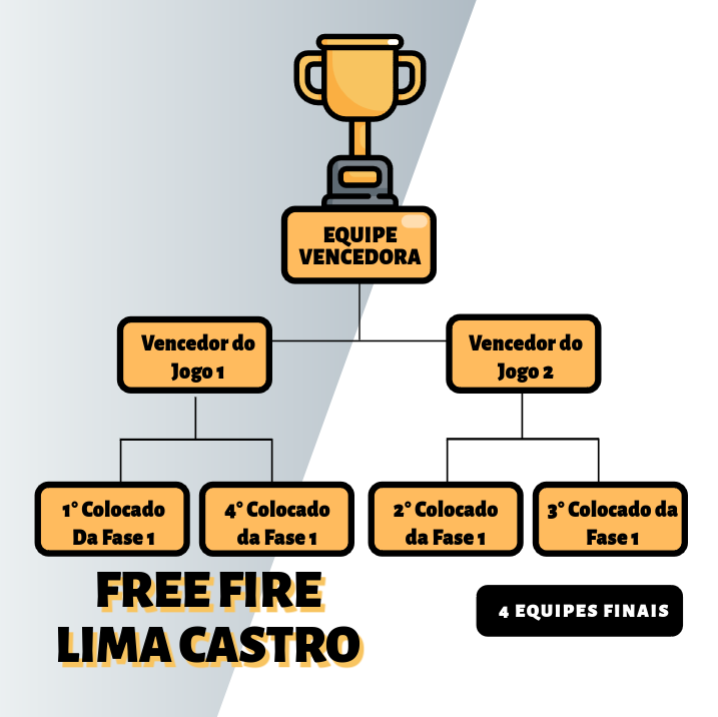
\includegraphics[width=.9\linewidth]{2-Imagens/bracket.png}
        \end{figure}

    \item As regras da segunda fase são:
        \begin{enumerate}[label={\bfseries \Roman* - }]
            \item As partidas serão disputadas com no máximo 13 rodadas;
            \item Não serão permitidos as seguintes armas: M1887, Double Vector, AWM e Granada;
            \item Não serão permitidos armas com atributos;
            \item Não serão permitidos os seguintes personanges: CR7 e Tatsuya;
            \item  Caso haja descrumpimento de alguma das normas, a equipe será automaticamente desclassificada.
        \end{enumerate}
\end{enumerate}

%----------------------------------------------------------------------
\section*{Do Calendário do Evento}

\begin{enumerate}[start=1,label={\bfseries Art. \arabic*$^\circ$ - }, resume]
    \item O campeonato acontecerá nos seguintes dias:
        \begin{enumerate}[label={\bfseries \Roman* - }]
            \item Primeira Fase: 09 de agosto de 2023 as 7:30h no horário matutino
                e as 13:00h no horário vespertino;
            \item Segunda Fase: 09 de agosto de 2023 as 11:00h no horário matutino
                e as 16:30 no horário vespertino.
        \end{enumerate}
    \item Segue abaixo o calendário do campeonato:

    \begin{center}
        Turno Matutino
    \end{center}
    \begin{multicols}{2}
        \begin{flushleft}
            \begin{tabular}{l l l}
                \hline
                \multicolumn{3}{c}{Primeira Fase - 9 de Agosto}\\
                \hline
                07:40h & Queda 1 & Mapa Bermuda \\
                08:30h & Queda 2 & Mapa Purgatório \\
                09:30h & Queda 3 & Mapa Kalahari\\
                \hline
            \end{tabular}
        \end{flushleft}

        \begin{flushleft}
            \begin{tabular}{l l l}
                \hline
                \multicolumn{3}{c}{Segunda Fase - 9 de Agosto}\\
                \hline
                11:00h & Final & Mapa Bermuda\\
                \hline
            \end{tabular}
        \end{flushleft}
    \end{multicols}

    \begin{center}
        Turno Vespertino
    \end{center}
    \begin{multicols}{2}
        \begin{flushleft}
            \begin{tabular}{l l l}
                \hline
                \multicolumn{3}{c}{Primeira Fase - 9 de Agosto}\\
                \hline
                13:50h & Queda 1 & Mapa Bermuda \\
                14:40h & Queda 2 & Mapa Purgatório \\
                15:50h & Queda 3 & Mapa Kalahari\\
                \hline
            \end{tabular}
        \end{flushleft}

        \begin{flushleft}
            \begin{tabular}{l l l}
                \hline
                \multicolumn{3}{c}{Segunda Fase - 9 de Agosto}\\
                \hline
                16:40h & Final & Mapa Bermuda\\
                \hline
            \end{tabular}
        \end{flushleft}
    \end{multicols}
\end{enumerate}

%----------------------------------------------------------------------
\section*{Da Integridade Competitiva}

\begin{enumerate}[start=1,label={\bfseries Art. \arabic*$^\circ$ - }, resume]
    \item Uso de BUG acarretará na desclassificação da equipe do campeonato.
    \item O uso de aplicativos que modifiquem o comportamento do jogo, conhecido
        como Hackers acarretará em desclassificação da equipe do campeonato.
    \item Será proibido todo e qualquer tipo de linguagem
        que contenha palavras obscenas, difamatórias, machistas, vulgares, libidinosas
        e/ou racistas que sejam ofensivas com o próximo e consigo mesmo.
\end{enumerate}

%----------------------------------------------------------------------
\section*{Da Interpretação e Atualização do Regulamento}

\begin{enumerate}[start=1,label={\bfseries Art. \arabic*$^\circ$ - }, resume]
    \item Todas as interpretações das regras, penalidades e demais decisões são prerrogativas
    da Comissão Organizadora.
    \item A falta de tipificação específica neste documento não impede que a
        Comissão Organizadora aja e tome decisões sobre qualquer assunto não previsto.
        No intuito de preservar a integridade competitiva, a Comissão poderá criar
        novas políticas complementares a este regulamento, incluindo, retirando ou
        alterando o conteúdo do mesmo.
    \item Os casos omissos serão resolvidos pela Comissão Organizadora, não
        podendo essas resoluções contrariar o Regulamento Geral.
\end{enumerate}
